\section{Исследование полей энерговыделения и теплогидравлических параметров при разных режимах работы реактора}

\subsection{Постановка задачи}
Необходимо провести анализ и расчет профиля энерговыделения в активной зоне а также основных теплогидравлических параметров, таких как температуры и давления теплоносителя, топлива, внешней и внуренней оболочки. В работе рассматриваются следующие режимы работы реактора:
\begin{itemize}
    \item На номинальной мощности
    \item На повышенной мощности
    \item При отключении одного из четырёх ГЦН
    \item При отключении двух их четырёх ГЦН
\end{itemize}

\subsection{Описание расчетного инструмента}
% TODO:
%   - [ ] мат модель
%   - [ ] дискретная модель
%   - [ ] про уравнение Пуассона 
Оценка энерговыделения и теплогидравлических параметров произведена с использованием програмного кода «ТРЕТОН». Данный инструмент разработан для расчета теплогидродинамических процессов в активной зоне реакторов типа ВВЭР. В нем реализованы алгоритмы многоуровневого решения уравнений теплообмена и гидродинамики.


\subsection{Расчет при работе на номинальной мощности}
Для первоначальной валидации програмного кода и подбора входных данных для дальнейшего анализа рассматриваемых режимов, произведем расчет температур при работе РУ на номинальной мощности.

Первым этапом необходимо определить распределение тепловыделения по всем расчетным элементам. Исходные расчетные элементы представляют собой 163 топливные ячейки ТВС. Для построения расчетной модели активная зона была разбита на 8 групп по радиусу от центра и на 30 зон по высоте, по которым были сгруппированы расчетные ячейки. Компоновка расчетных ячеек и разбиение по группам представлены на картограмме \ref{pic:treton-kartogramma}


\begin{figure}[H]
	\begin{center}
		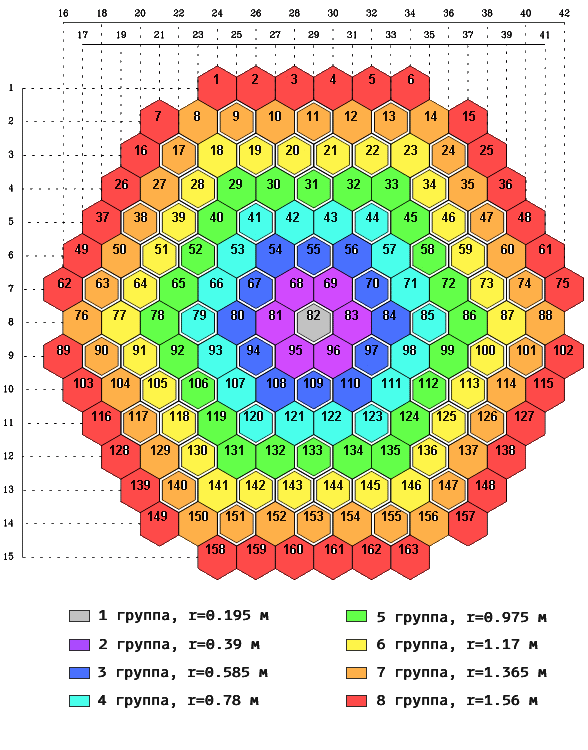
\includegraphics[scale=0.7]{treton_cells.png}
		\caption{Картограмма ячеек моделируемой АЗ для расчетного кода «ТРЕТОН» и их разбиение на группы по радиусу}
		\label{pic:treton-kartogramma}
	\end{center}
\end{figure}


Для каждой зоны были расчитаны тепловыделения, нормируя на соответствующие $K_r^i$, $K_z^j$, где $i = \overline{1, 8}$, $j = \overline {1, 30}$.

Распределение $K_r$ по группам было подобрано ориентируясь на следующие зависимости:
\begin{equation}
    K_r(r) \sim J_0(\frac{\xi_0 r}{R_{\text{эфф}}}) \approx - \alpha r^2 + \beta
\end{equation}, распределение коэффициента неравномерности по радиусу в приближении параболической функции
\begin{equation}
    \label{equation:KriNi}
    \sum_{i=1}^{8} K_r^i N_i = N_{\text{ТВС}} \pm 0.01
\end{equation}, где $N_i$ — количество ТВС в $i$-той группе по радиусу – условие нормировки распределения коэффициента неравномерности по радиусу.
Коэффициент $\beta$ параболической функции был подобран из условия, что в центре $K_r(r=0)$ должна быть равна табличному значению $K_r$ из \ref{tabular:data}, коэффициент $\alpha$ для удовлетворения соотношения \ref{equation:KriNi}. Полученные значения распределения коэффициента неравномерности по радиусу для каждой группы представлены в таблице \ref{tabular:Kri}.

\begin{figure}[H]
	\begin{center}
		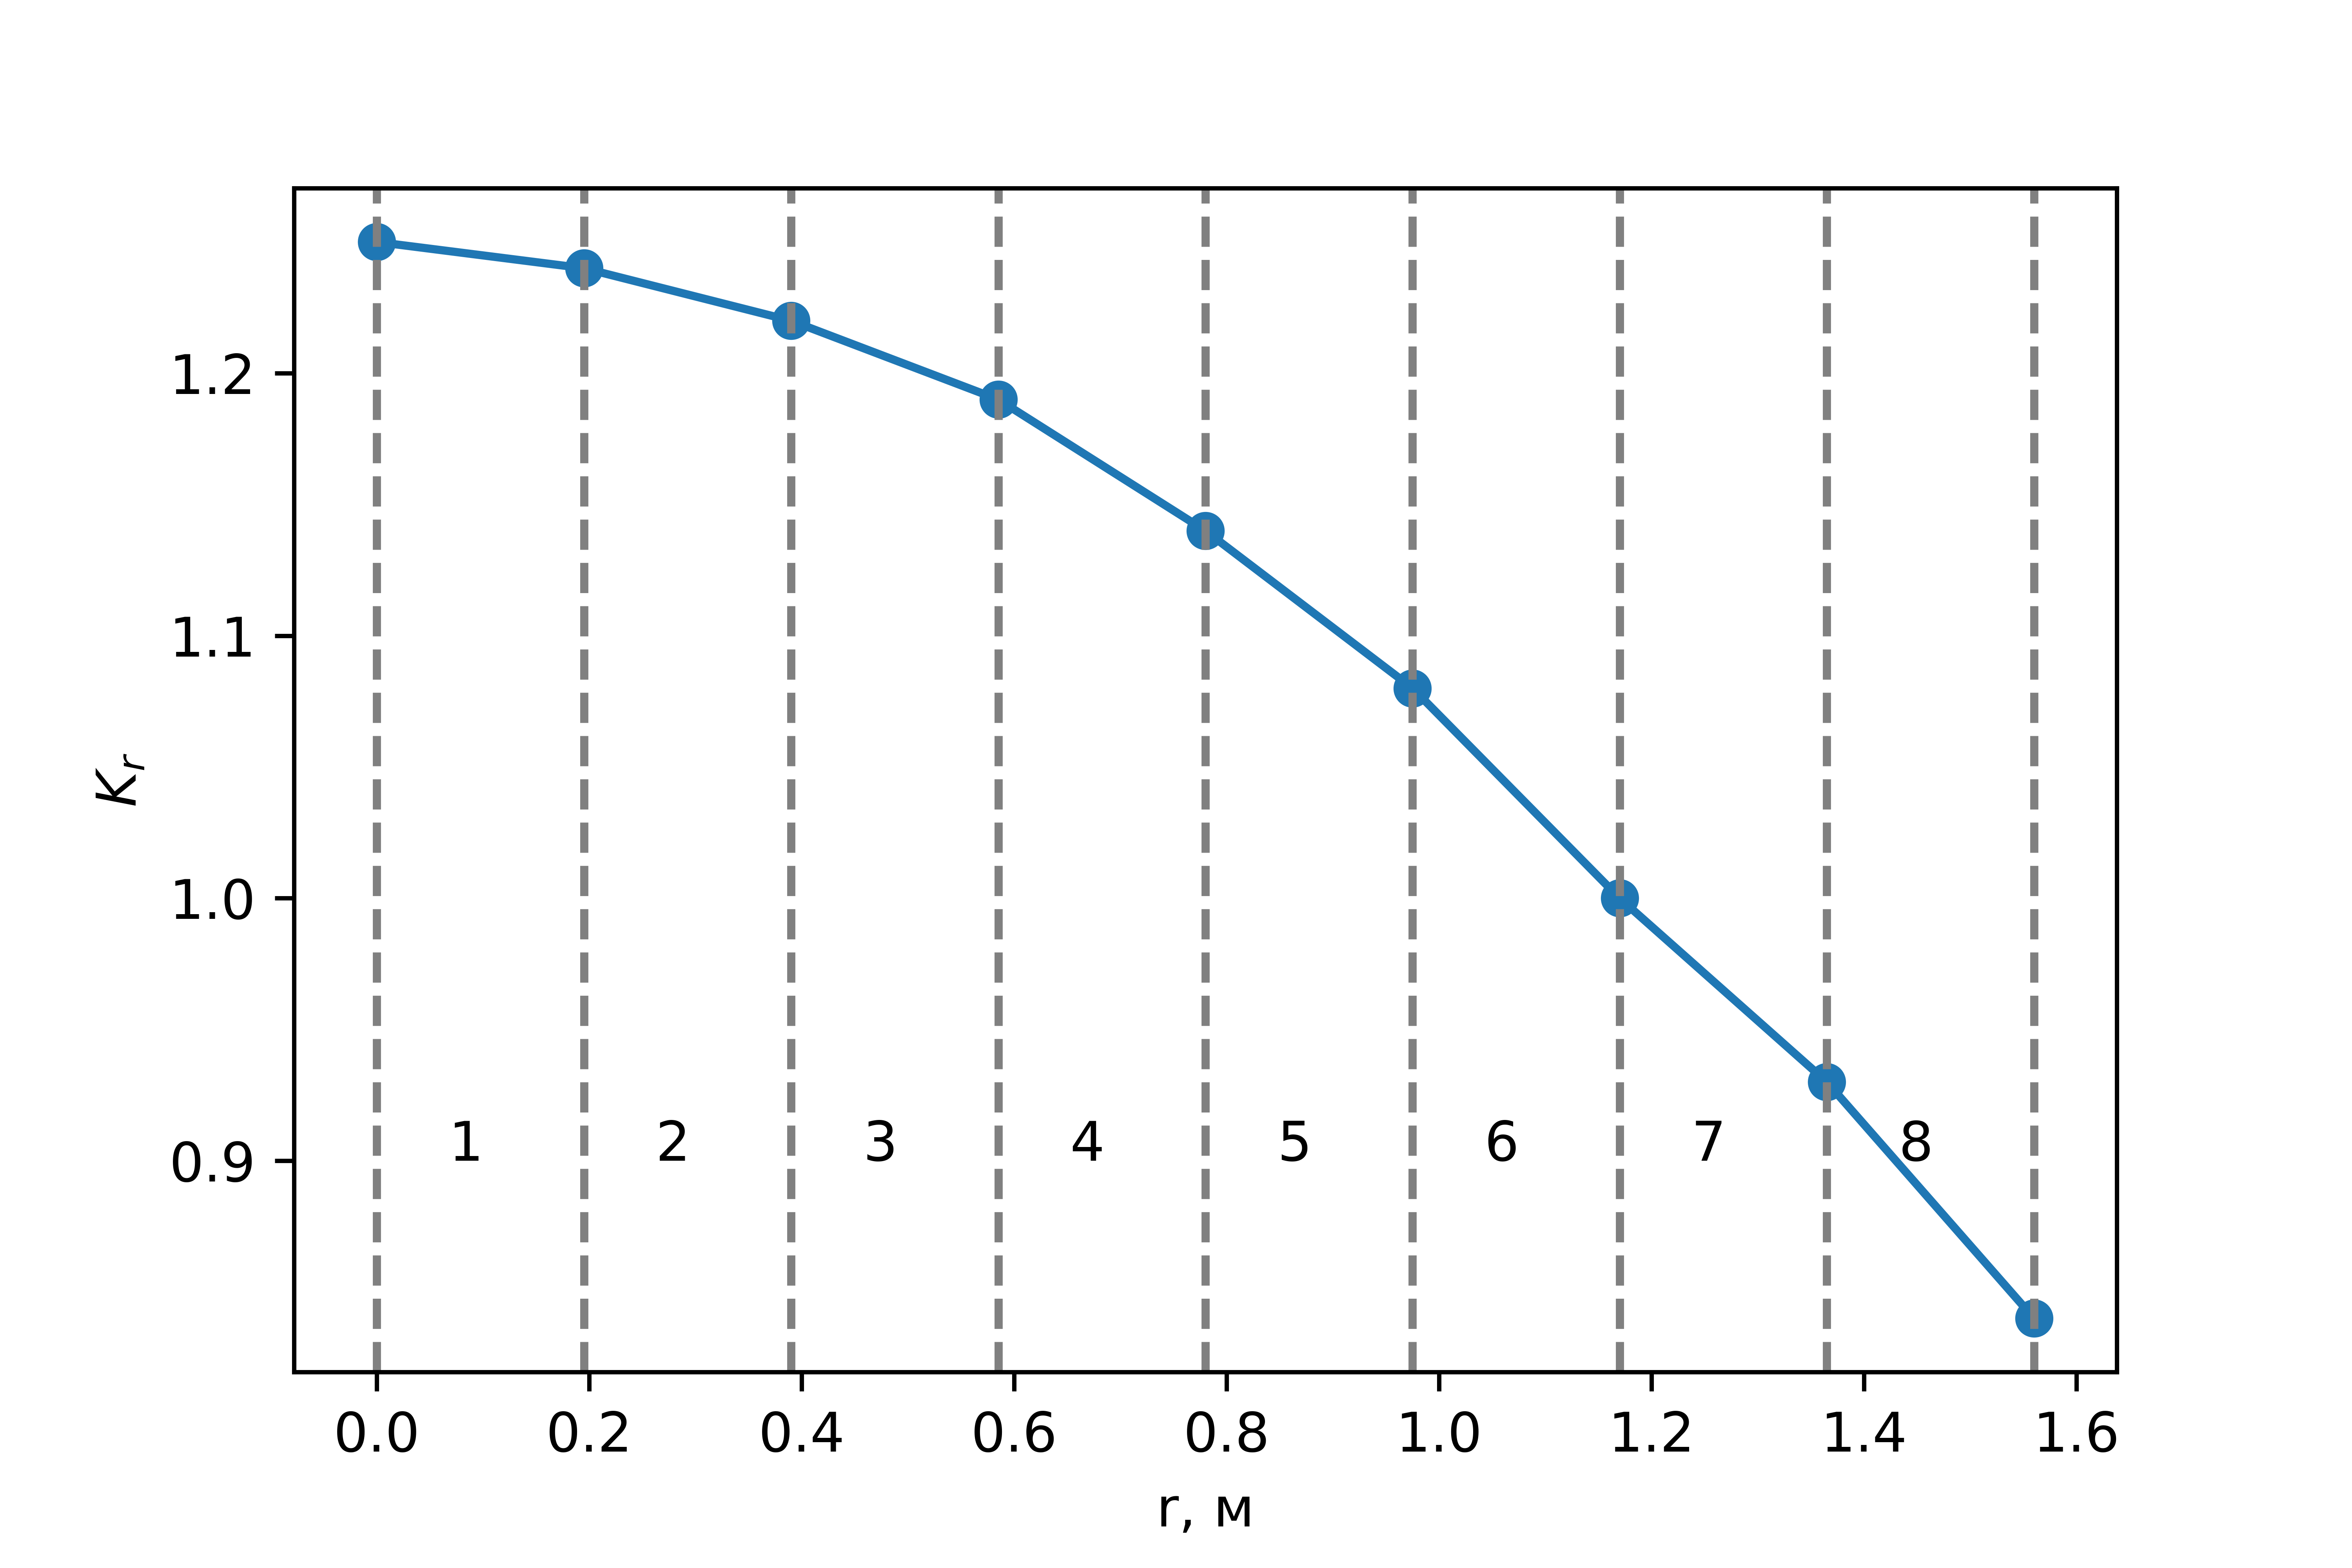
\includegraphics[scale=0.8]{Kr.png}
		\caption{Распределение коэффициента неравномерности по радиусу для восьми групп ТВС}
		\label{pic:Kr}
	\end{center}
\end{figure}

\begin{table}[H]
	\caption{Коэффициент неравномерности энерговыделения по радиусу для групп ТВС}
	\begin{center}
        \begin{tabular}{|l|c|}
        \toprule
         Номер группы & Значение $K_r^i$ \\
         \midrule
         \hline
         1 & 1.24 \\
         \hline
         2 & 1.22 \\
         \hline
         3 & 1.19 \\
         \hline
         4 & 1.14 \\
         \hline
         5 & 1.08 \\
         \hline
         6 & 1.00 \\
         \hline
         7 & 0.93 \\
         \hline
         8 & 0.84 \\
         \bottomrule
		\end{tabular}
		\label{tabular:Kri}
	\end{center}
\end{table}


\noindent Распределение коэффициента неравномерности по высоте $K_z$ определяется как:
\begin{equation}
    K_z(z) = K_z \cos \left( \frac {\pi z} {H_{\text{эфф}}} \right)
\end{equation}
где $z = \overline{-H_{\text{АЗ}} / 2,\  H_{\text{АЗ}} / 2}$ м.


\noindent Распределение $K_z$ по высоте представлено на рис \ref{pic:Kz}


\begin{figure}[H]
	\begin{center}
		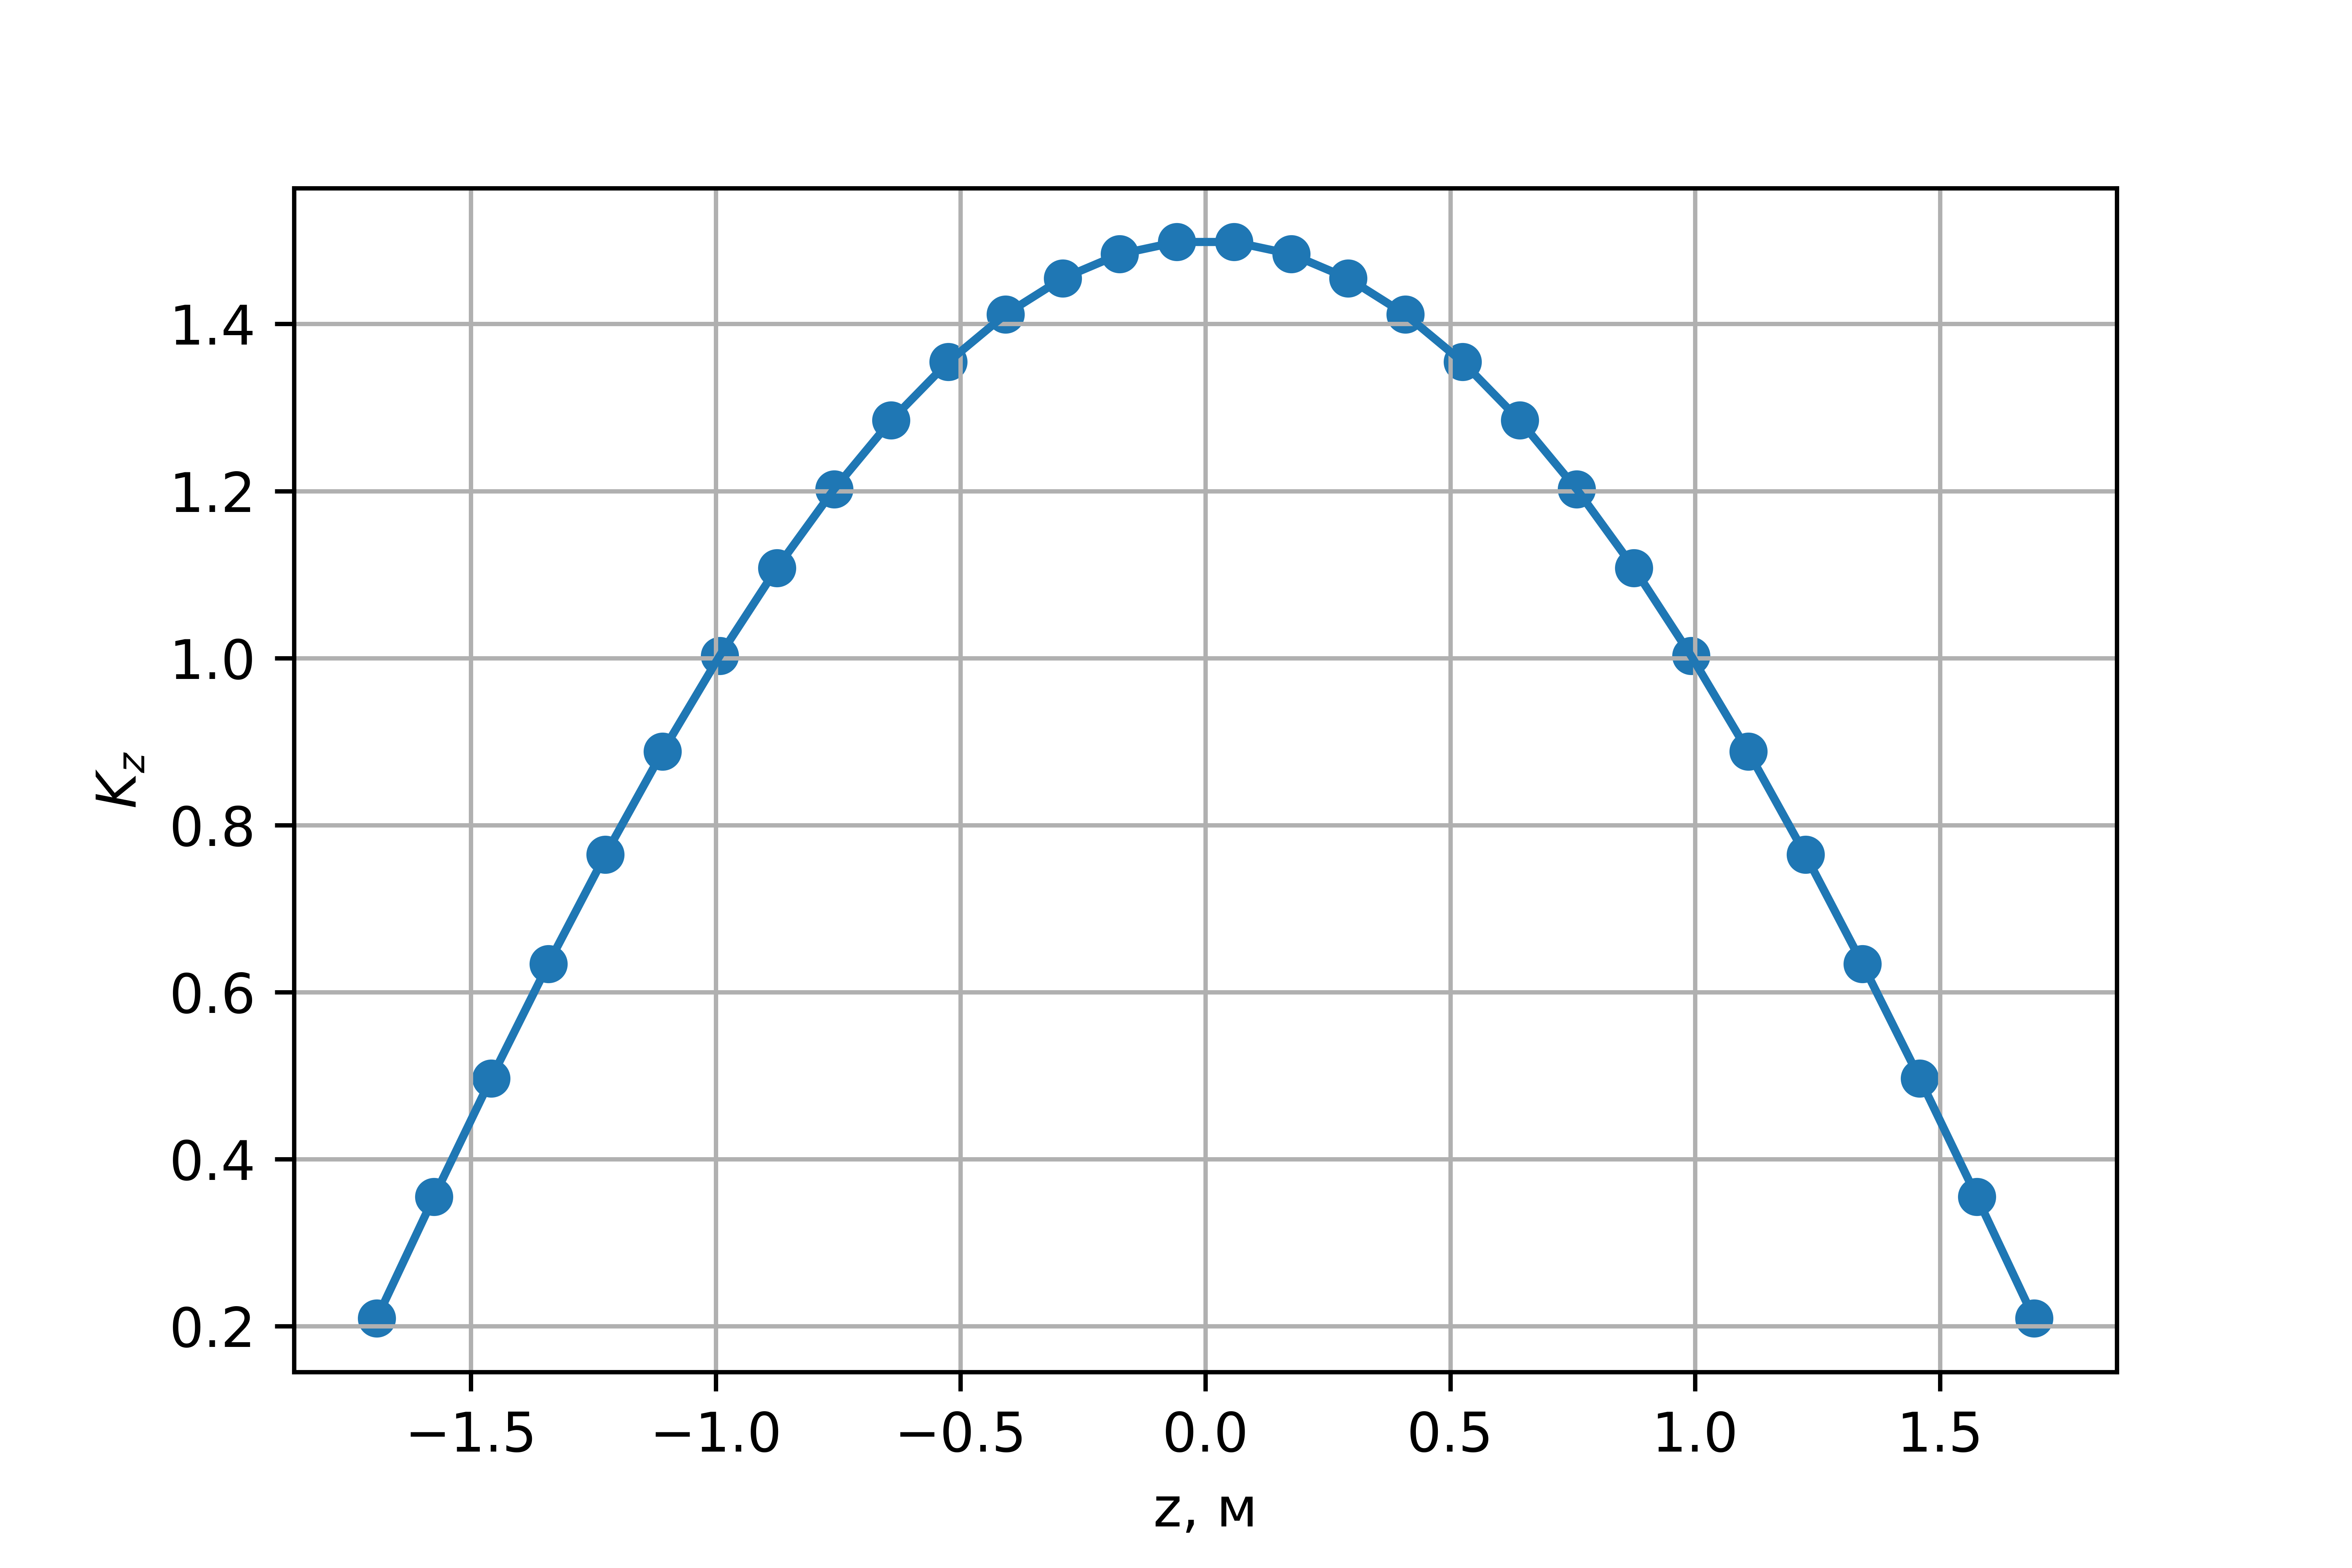
\includegraphics[scale=0.8]{Kz.png}
		\caption{Распределение коэффициента неравномерности по высоте активной зоны}
		\label{pic:Kz}
	\end{center}
\end{figure}


Из полученных распределений $K_r$, $K_z$ было определено распределение тепловыделения для всех групп расчетных элементов
\begin{align}
    \label{equation:Qzr}
    Q(z, r) &= K_z(z)K_r(r)\frac{Q_{\text{теп}}}{N_{\text{ТВС}} \cdot 30} \\
            &= K_r(r) K_z \cos \left( \frac{\pi z}{H_{\text{эфф}}} \right) \frac{Q_{\text{теп}}}{N_{\text{ТВС}} 30}
\end{align}

На основе соотношения \ref{equation:Qzr} был сформирован входной файл \texttt{Q6.txt} с тепловыделением для всех расчетных элементов в соответствии с картограммой \ref{pic:treton-kartogramma}

Далее были проведены калибровочные расчеты для определения входных параметров файла \texttt{THEHYCO.INI}, соответствующих проектируемой РУ. Основным критерием выбора параметров было соответсвие вычисленному программой «ТРЕТОН» расходу полученному ранее в рамках теплофизического расчета.

Таким образом расчетным кодом было получено значение расхода $G_{\text{расч}} = (1.570 \pm 0.016) \cdot 10^4\  \frac{\text{кг}}{\text{с}}$, что соответствует полученному ранее значению $G_{\text{реак}} = 1.579 \cdot 10^4\ \frac{\text{кг}}{\text{с}}$ в пределах погрешности. 
Значения входных параметров файла \texttt{THETHYCO.INI}, при которых достигнут такой расход приведены в таблице % \ref{tabular: thethyco_nominal}

\begin{table}[H]
    \caption{Входные параметры расчета при номинальном режиме работы}
    \begin{center}
        \begin{tabular}{|l|c|}
        \toprule
        Параметр & Значение \\
        \midrule
        \hline
        Шаг твэлов, мм & 12.75 \\ 
        \hline
        Поперечный размер расчетной области, м & 0.241 \\
        \hline
        Продольный размер расчетной области, м & 0.118 \\
        \hline
        Кол-во твэлов в ТВС, шт & 317 \\
        \hline
        Расчетный дисбаланс & 0.005 \\
        \hline
        Входное давление, Па & 15800000 \\
        \hline
        Выходное давление, Па & 15686938 \\
        \bottomrule
        \end{tabular}
    \end{center}
\end{table}

% TODO: табличка с параметрами THEHYCO.INI по разделам с именами

% \begin{table}[H]
% 	\caption{wow}
% 	\begin{center}
%         \begin{tabular}{|l|c|}
%         \toprule
%          Раздел RodList & \\
%          \midrule
%          \hline
%          tmp=0.75 3.86 4.25 4.55 & разбиение твэлов на контрольные объемы, указаны радиусы центрального отверстия твэла, границы топливного столба, центра оболочки, внешней границы оболочки. мм\\
%          \hline
%          $\texttt{s_mesh}$=12.75 & шаг твэлов, мм \\
%          \hline
%          d\_mesh=9.1 & диаметр твэла, мм \\
%          \hline
%         %  $\texttt{R_contact}$=0.00024 & контактное сопротивление толиво-оболочка, $\text{м}^2 \cdot \text{К} / \text{Вт}$ \\
%         %  \hline
%          Раздел HEATandHYDROlist & \\
%          \midrule
%          \texttt{dr}=0.241 & поперечный размер расчетной области, м\\
%          \hline
%          \texttt{dz}=0.118 & продольный размер расчетной области, м\\
%          \hline
%          $\texttt{n_RodsInTVS}$ =317 & количество твэлов в ТВС \\
%          \hline
%          \texttt{Disbalance}=0.001 & расчетный дисбаланс \\
%          \hline
%          $\texttt{p_input}$=15800000 & входное давление, Па \\
%          \hline
%          $\texttt{p_output}$=15691054 & выходное давление,  Па \\
%          \bottomrule
% 		\end{tabular}
% 		\label{tabular:thehyco_nominal}
% 	\end{center}
% \end{table}

На основе описанных входных параметров был произведен расчет с шагом по времени $dt=0.0005$ для 100 итераций. По результату расчета были построены зависимости основных теплогидравлических параметров и сопоставлены со значениями, полученными в тепло-физческом расчете.

\noindent Распределение температуры теплоносителя по высоте активной зоны для кассеты с максимальной температурой теплоносителя на выходе из активной зоны
